\documentclass[ignorenonframetext]{beamer}
\usepackage{textpos}
\usepackage{graphicx}
\usepackage{pgf}
\usepackage{listings}
\usepackage{multimedia}
\usepackage{gensymb}
\usepackage{amsmath, mathrsfs}
\usepackage{adjustbox}
\usepackage{tikz}
\usepackage{tikz-3dplot}

\usetikzlibrary{shapes.geometric, arrows.meta, calc}

% \captionsetup[figure]{labelformat=empty}% redefines the caption setup of the figures environment in the beamer class.

\lstdefinestyle{yaml}{
     basicstyle=\ttfamily\color{blue}\tiny,
     rulecolor=\color{black},
     string=[s]{'}{'},
     stringstyle=\color{blue},
     comment=[l]{:},
     commentstyle=\color{black},
     morecomment=[l]{-}
 }

\usetheme{Boadilla}
\usefonttheme{serif}
% \mode<presentation>
% {
%  \usefonttheme{serif}
% % \useoutertheme{sidebar}
% %   \logo{\includegraphics[height=1cm]{elec_logo.pdf}}
% }

\title[TART Position Cal]{Antenna Array Position Calibration for the Transient Array Radio Telescope}

\author[Molteno]{Tim Molteno}

\institute[Otago]
{
  Electronics Research Foundation, New Zealand \\
  \& \\
  Dept of Physics,
  University of Otago, New Zealand \\
  \& \\
  Dept of Physics \& Electronics,
  Rhodes University, South Africa \\
  \vspace{1cm}
  \vspace{2cm}
  \includegraphics[width=0.6\linewidth]{fig/elec_header_font.pdf}
}

\logo{\pgfputat{\pgfxy(-0.72,7.7)}{\pgfbox[center,base]{\includegraphics[width=1cm]{fig/elec_logo.pdf}}}}

\date[TART Mada 2026] % (optional, should be abbreviation of conference name)
{}

% \addtobeamertemplate{headline}{}{%
% \begin{textblock*}{100mm}(0.87\textwidth,2mm)
% \includegraphics[height=1.5cm]{elec_logo.pdf}
% \end{textblock*}}

\begin{document}


%opening


\begin{frame}
  \titlepage
\end{frame}




\begin{frame}
 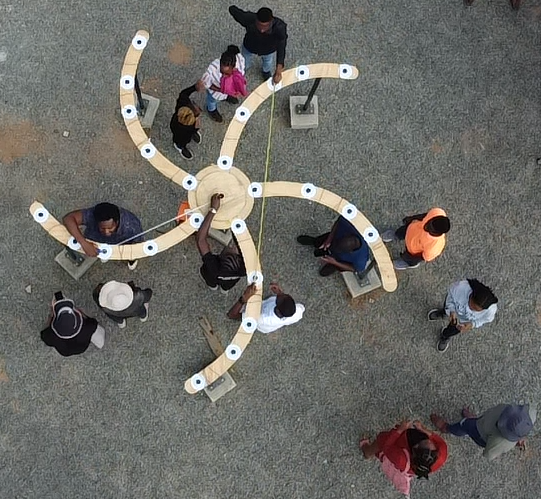
\includegraphics[width=\linewidth]{fig/botswana_calibration.png}
 Aerial view of a TART being calibrated by attendees at a TART workshop hosted at the Botswana International University of Science and Technology, in March 2025.
\end{frame}

The calibration process must involve easy-to-make measurements, and be robust to accidental errors in measurement. This paper outlines an iterative calibration process that meets these requirements.

\section{Method}

The process involves measuring two kinds of distances. The first are the {\em radial distances} between the phase-centre and the centre of each antenna. There are 24 radial distance measurements $r_i$. The second measurements are the pairwise distances between each pair of antennas. There are $\frac{1}{2} N (N-1)$ unique pairs of antennas for an array with $N$ antennas. For the TART there are 276 pairwise distances $\delta_{ij}$ between antennas $i$ and $j$. As the measurements do not constrain the global rotation of the array, it is assumed that the direction between the phase centre and one of the antennas is known. This direction is the measured angle between one antenna and geographic North.

\begin{frame}{Method}
 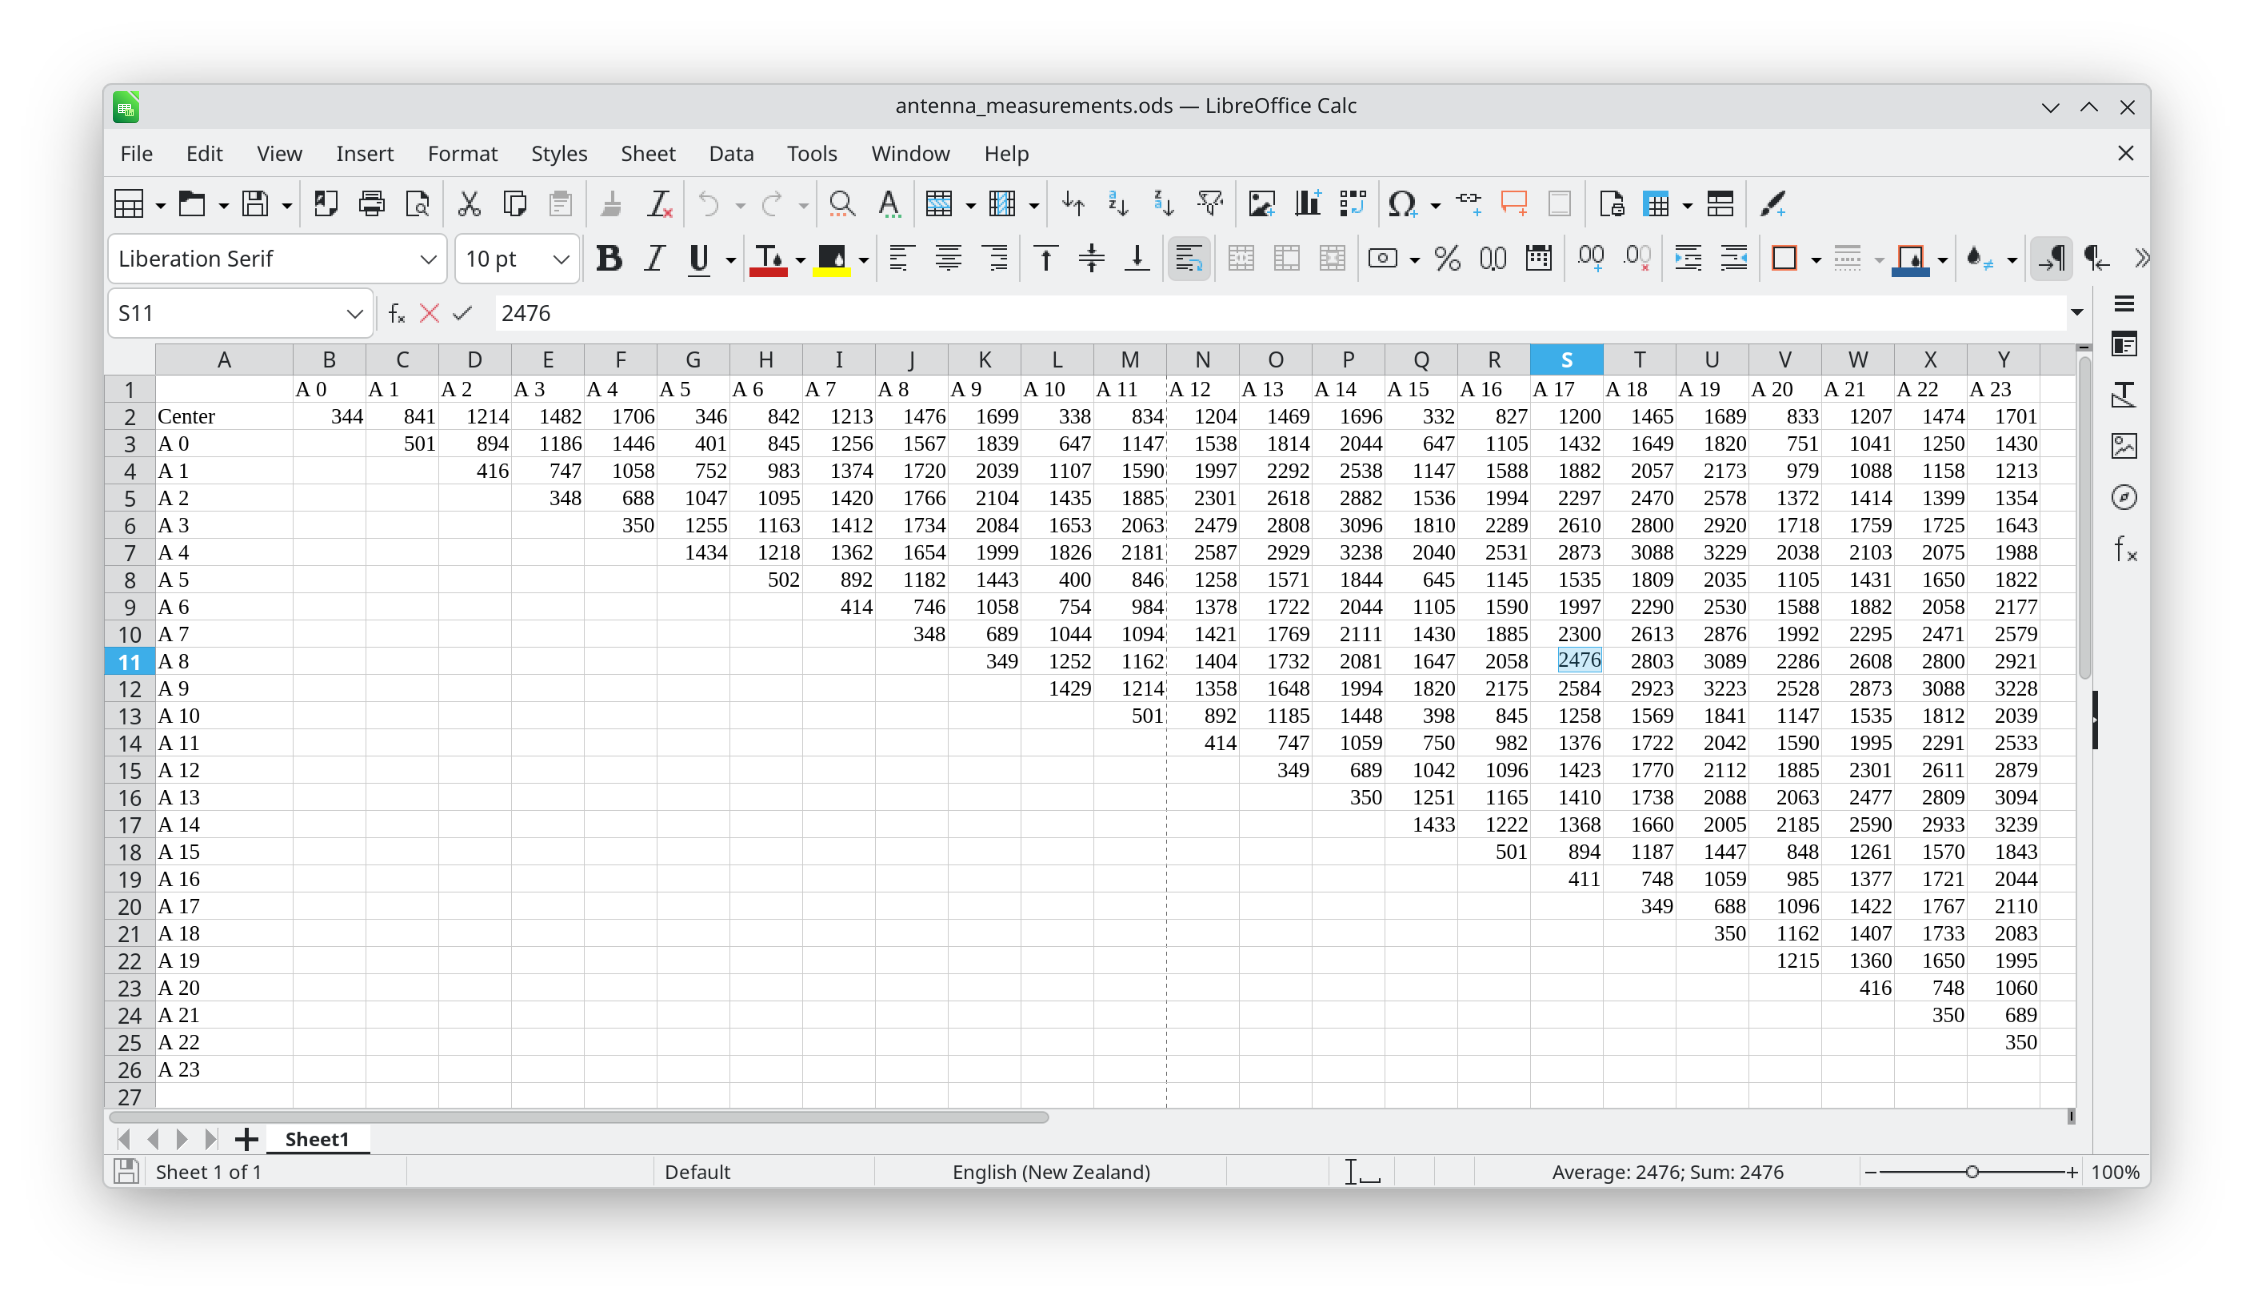
\includegraphics[width=\linewidth]{fig/spreadsheet.png}
 Spreadsheet with the measurements from a TART antenna array. The highlighted entry shows the distance in mm, between antenna 17, and antenna 8.
\end{frame}

The purpose of the algorithm is to estimate the 24 antenna positions in the $x-y$ plane that are most consistent with the measurements.

\begin{frame}{Least Squares Estimator}

Given a set, $x,y$ of 24 antenna positions, and the $r_i, \delta_{ij}$, we form a least-squares estimator

\begin{eqnarray}
 L_{}(x, y) & = & L_r(x,y) + L_{ij}(x,y) \\
 & = & \sum_{i=1}^{N} \left( r_i - \sqrt{x_{i,0}^2 + y_i^2}  \right)^2 \nonumber \\
 & + & \sum_{i,j=1}^{N} \left( \delta_{ij} - \sqrt{(x_i - x_j)^2 + (y_i - y_j^2}  \right)^2
\end{eqnarray}
\end{frame}

Where one set of residuals corresponds to the radius measurements $r_i$, and the other set of residuals corresponds to the measured distances $\delta_{ij}$ between antennas.

\subsection{Algorithm}

The algorithm starts with a set of {\em initial estimates} of $x_i, y_i$, the coordinates of the $i$th antenna. From these, the simulated measurements $r^s_i = \sqrt{x_i^2 + y_i^2}$, and $\delta^s_{ij} = \sqrt{(x_i - x_j)^2 + (y_i - y_j^2}$ are calculated. The least squares estimator $L(x,y)$ is then minimized (as a function of $x_i, y_i$) to find the set of antenna positions that produce simulated measurements that are as close as possible to the actual measurements.

\begin{frame}{The end result}
 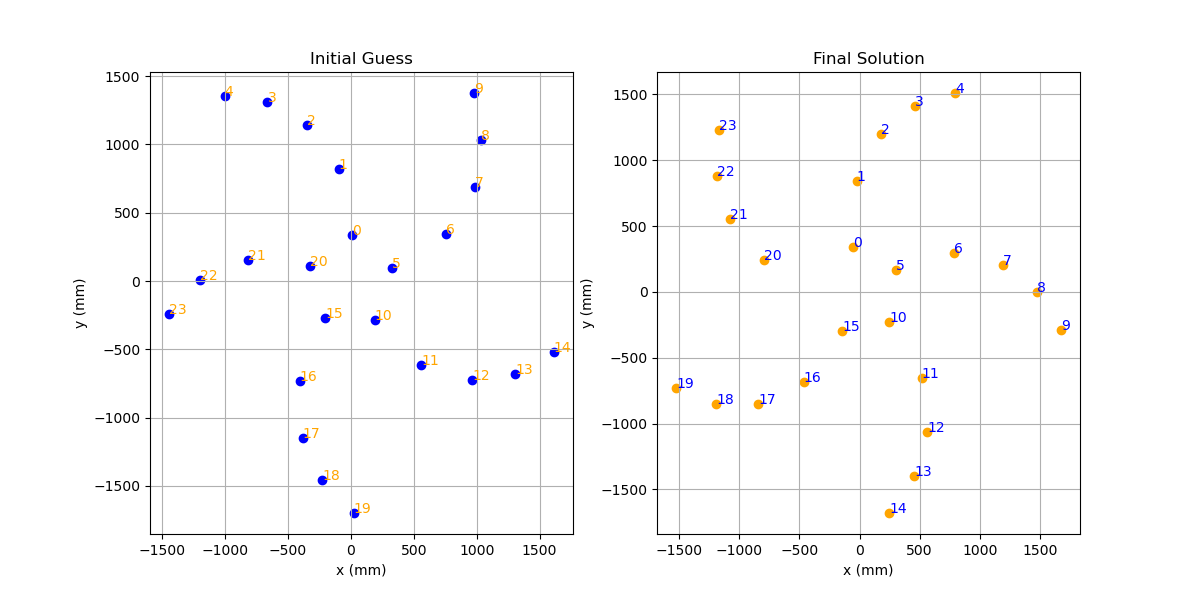
\includegraphics[width=\linewidth]{fig/final_positions.png}
 Initial position estimates, and the final positions for the TART antenna array after calibration.
\end{frame}

\begin{frame}{Residuals}

\begin{columns}
 \begin{column}{0.5\linewidth}
 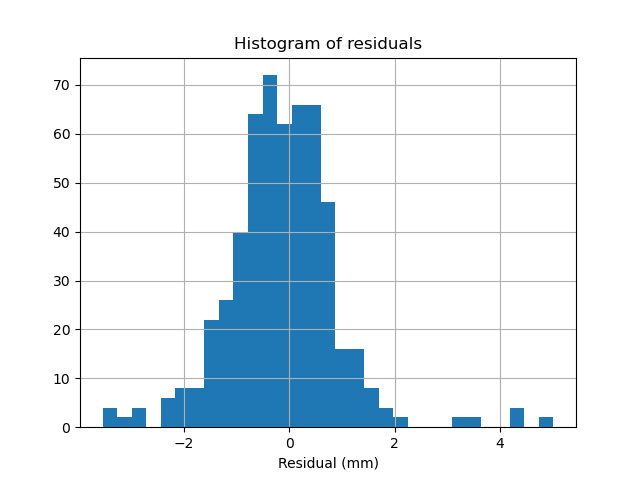
\includegraphics[width=\linewidth]{fig/residual_histogram.png}
  90th percentile of residuals is 1.53 mm
 \end{column}
 \begin{column}{0.5\linewidth}
The differences between the simulated measurements of the calibrated positions, and the actual measurements made are called residuals. If one or more of the residuals are large, it usually indicates a measurement error, and these large residuals can be used to re-check just a few of the measurements.

 \end{column}
\end{columns}


\end{frame}

\end{document}
